\chapter{Approfondimento C}
\section{Funzioni di Libreria}
\subsection{Assert}
Cominciamo dicendo che \texttt{assert} non è una funzione di libreria,
anche se viene utilizzata nello stesso modo, ma è una \textbf{macro}. 
Essa prende in ingresso un'espressione e, se questa risulta falsa,
interrompe l'esecuzione del programma. Per utilizzarla:
\begin{verbatim}
#include <assert.h>
assert(exp); // espressione da valutare
\end{verbatim}
L'\texttt{assert} serve tipicamente per il \textbf{debug} e per verificare condizioni
interne del programma. In caso di errore, il programma viene terminato
(chiamando \texttt{abort()}).Se è definito \texttt{NDEBUG}, gli \texttt{assert} 
vengono disabilitati e non hanno effetto.
\subsection{Funzioni per la gestione di Stringhe}
Dato che C non offre delle funzioni per la gestione delle stringhe
è molto utile utilizzare delle funzioni esterne in base alle nostre esigenze,
come:
\begin{verbatim}
#include <string.h>
size_t strlen(const char* s);                          // calcola la lunghezza della stringa
char* strcpy(char *dst, const char* src);              // copia la stringa in un altra stringa
char* strncpy(char *dst, const char* src, size_t len); // copia la stringa fino al len 
                                                          carattere da src in dst. Se src
                                                          è più piccolo di dst i verranno riempiti
                                                          con il carattere '/0'. Mentre in caso 
                                                          di dst è più piccolo di src i 
                                                          caretteri andranno persi.
char* strcat(char* dst, const char* src);              // concatena le due stringhe
\end{verbatim}
\textbf{\textcolor{red}{ATTENZIONE:}} \texttt{dst} deve contenere abbastanza spazio
libero per contenere src
\begin{verbatim}
char* strtok(char* src, const char* delim); // divide la stringa in token
\end{verbatim}
Utilizzo:
\begin{verbatim}
    char* tocken= strtok(str, delim);
    while(token != null){
        .... codice che fa qualcosa con tocken
        tocken = strtok(NULL, delim);           // per andare al prossimo tocken
    }
\end{verbatim}
Vediamo però come funziona ogni parametro:
\begin{figure}[H]
    \centering  
    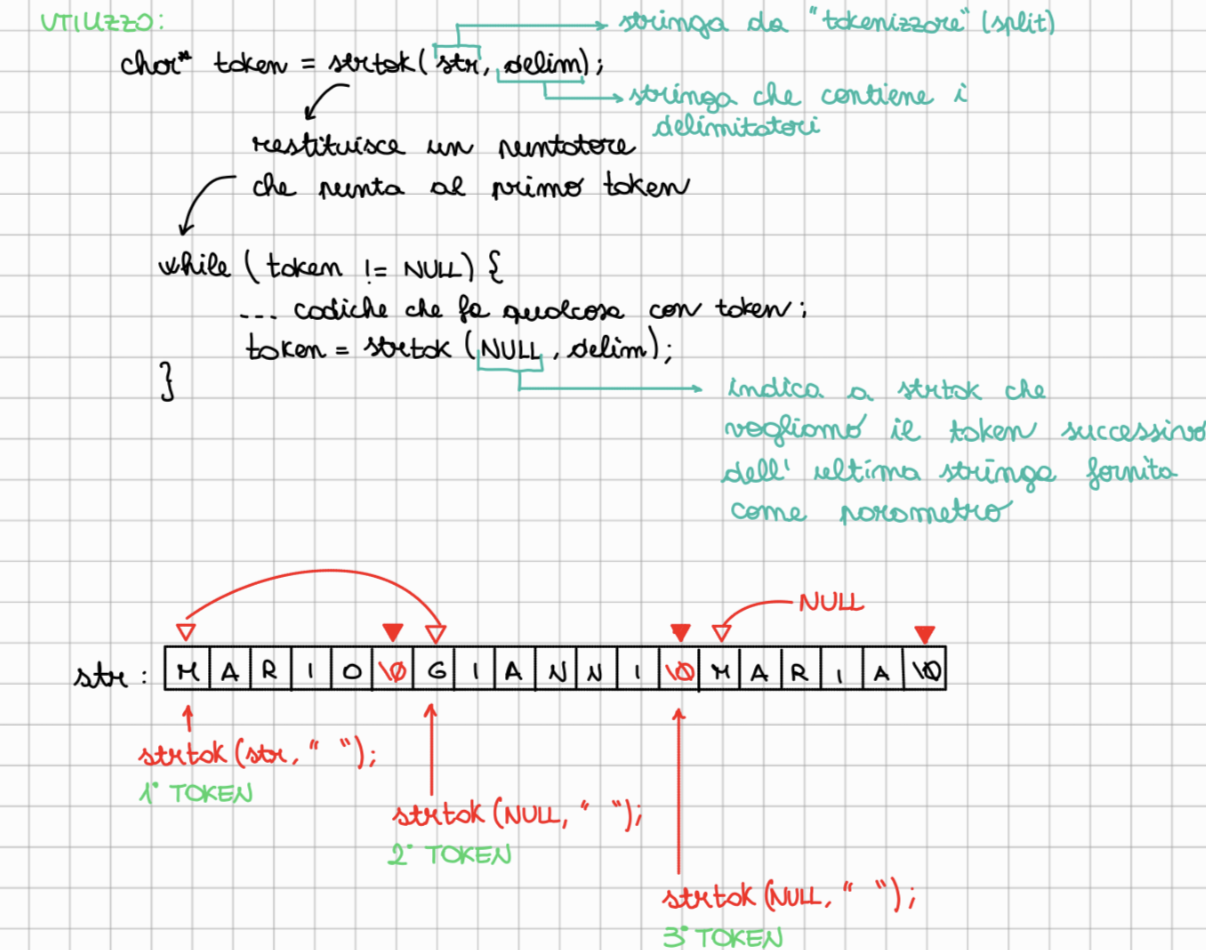
\includegraphics[width=0.9\linewidth]{../images/strtok.png}
    \caption{Funzionamento token}
    %\label{label}
\end{figure}
\noindent Vediamo ora un esempio di utilizzo:
\begin{verbatim}
    #DEFINE DELIM = ", "
    
    char* f(const char* s){
        char* temp = NULL;
        char* res = NULL;
    
        size_t len = strlen(s);
        char* tempo = malloc(sizeof(char)*(len+1));
        if(temp == NULL) goto cleanup;
        strncpy(temp, s, len);
        
        char* res = malloc(sizeof(char)*(len+1));
        if(res == NULL) goto cleanup;
        
        char* token = strtok(temp, DELIM);
        while(token){
            strncat(res, token, strlen(token));
            token = strtok(NULL, DELIM);
        }

        free(temp);
        retun res;
                
        cleanup:
        if(temp != NULL) free(temp);
        if(res != NULL) free(res);
        return NULL;
    }
\end{verbatim}
Utilizziamo il "\#DEFINE DELIM" per definire i delimitatori, in modo da 
non doverli riscrivere e poterci confondere.\medskip\\
Procediamo col vedere altre funzioni presenti nella libreria \texttt{string.h}:
\begin{verbatim}
int strcmp(const char* s1, const char* s2);
\end{verbatim}
Questa funzione confronta s1 ed s2 e restituisce: \medskip\\
$
\begin{cases}
    \textbf{$<$0} \text{        se s1 precede s2} \\
    \textbf{0}    \text{        se } s1 == s2 \\
    \textbf{$>$0} \text{        altrimenti}
\end{cases}
$\bigskip\\
Passiamo alla libreria \textbf{stdlib.h}:
\begin{verbatim}
#include <stdlib.h>
int atoi(const char* s); // converte s in un valore intero se possibile, altrimenti restituisce 0
\end{verbatim}
Esempio:
\begin{verbatim}
atoi("10");     --> 10
atoi("10abc");  --> 10
atoi("abc10");  --> 0 perchè non inizia con un numero
atoi("-10");    --> -10
\end{verbatim}
Esempio basilare di utilizzo:
\begin{verbatim}
void f(char* in[], int out[], int n){
    for(int i=0; i<n; i++)
        out[i] = atoi(in[i]);
}
\end{verbatim}
Vediamo ora degli esercizi dove otteniamo il minimo della lunghezza di due stringhe 
e un esercizio che verifica se un array di stringhe è ordinato o meno, utilizzando le funzioni viste
precedentemente:
\begin{verbatim}
int min_len(const char* a, const char* b){
    if(strlen(a)>=strlen(b))
        return strlen(a);
    else return strlen(b);
}

int is_sorted(char *v[], int n){
    for(int i=1; i<n; i++)
        if(strncmp(v[i-1], v[i], min_len(v[i-1], v[i])) > 0) return -1;
    return 0;
}
\end{verbatim}
Passiamo ora alal libreria \textbf{stdio.h}:
\begin{verbatim}
#include <stdio.h>
int sscanf(const char* s, const char* format, ...); 
\end{verbatim}
Questa funzione è simile a \texttt{scanf}, ma invece di leggere da standard input, legge da una stringa. 
Il primo parametro è la stringa da cui leggere, il secondo è il formato da utilizzare per la lettura, 
e i successivi sono i puntatori alle variabili dove salvare i valori letti.\\
Abbiamo poi la funzione \texttt{sprintf} che è simile a \texttt{printf}, ma invece di scrivere su standard output, scrive su una stringa.
Che fa sempre parte della libreria \textbf{stdio.h}:
\begin{verbatim}
int sprintf(char *d, const char* format, ...);
\end{verbatim}
Questa funzione scrive in d la stringa format formattata con i valori passati come argomenti, quindi:
il primo parametro è la stringa dove scrivere, il secondo è il formato da utilizzare per la scrittura, 
e i successivi sono i valori da scrivere.\\
Vediamo un esempio di utilizzo:
\begin{verbatim}
// converte una data da formato (input) "gg/mm/aaaa" a "mm/gg/aaaa"
int convert_date(const char *input, const char *output){
    int a,b,c;
    int res = sscanf(input, "%d/%d/%d", &a, &b, &c);
    if (res < 3) return -1;
    sprintf(output, "%d/%d/%d", b, a, c);
}
\end{verbatim}
Vediamo ora \texttt{getchar()}:
\begin{verbatim}
int getchar();                      // legge un carattere da standard input (da tastiera) 
                                        e lo restituisce come intero
int scanf(const char* format, ...); // legge da tastiera e salva i valori letti nelle 
                                        variabili passate come argomenti
\end{verbatim}